\documentclass[11pt,a4paper]{article}
\usepackage[top=2cm,left=2cm,right=2cm,footskip=0.75in]{geometry}
\usepackage{graphicx}
\usepackage{floatrow}
\usepackage{amsmath,amssymb}
\usepackage{url}
\usepackage[utf8x]{inputenc}
\usepackage{setspace}
\setstretch{1.1}
% \usepackage[document]{ragged2e}
\setcounter{section}{26}  % this is a section 27 of the proposal form

% \setlength{\oddsidemargin}{0.25in}
% \setlength{\textwidth}{6.5in}
% \setlength{\topmargin}{0in}
% \setlength{\textheight}{8.5in}

\usepackage{fontspec}
\setmainfont{Calibri}

% \usepackage{fontspec}
% \setmainfont[Path=/System/Library/Fonts/,
%     BoldItalicFont=calibriz.ttf,
%     BoldFont      =calibrib.ttf,
%     ItalicFont    =calibrii.ttf]{calibri.ttf}

\renewcommand{\bold}{\textbf}
\graphicspath{ {./images/} }

\begin{document}

\title{\large Computational Toolbox for Discovery of Prognostic Markers in Survival Analysis from Gene Expression Data: Description of the Research Project}
\author{}
\date{}
\maketitle
\vspace*{-1cm}

We propose a project to design and develop an interactive, visualization-based exploratory analysis toolbox to assist in finding molecular prognostic biomarkers from high-throughput biomedical survival data. The project will devise computational and machine learning methods to search for biomarkers, encapsulate them within interactive components with graphical user interface, and provide visual programming to stitch these components into data analysis pipeline. The constructed methods and toolbox will support collaborations between the data scientists and domain experts – physicians, biomedical or pharma researchers – to sip through the molecular cell-response data of thousands of genes to find those that most influence the survival. The proposed tool will access existing models, ontologies, and knowledge bases to speed-up the analysis process and provide automatic explanations of results. 

This is an applied project where we are teaming up with Genialis, a data science company specializing in computational support for precision medicine. The proposed set of methods, tools, and experience gained through the project will help Genialis obtain a cutting-edge in the biomarker discovery field, improve communication of their data analysis results to their customers, and increase their competitiveness. It will allow us, the proposing institution, to further advance our research in combination of interactive visualizations and machine learning, and apply our new approaches to a challenging field of biomarker discovery.

\subsection{Scientific background, problem identification and objectives of the proposed research}



\subsubsection*{Scientific Background}

\bold{The project will contribute new methods and practical data exploration approaches to the field of survival analysis and study how covariates jointly affect the changes in the survival functions.} Survival analysis is a set of statistical methods aimed at determining the life expectancy of the investigated population. Survival analysis studies the expected duration of time until an event, say, a cancer relapse after chemotherapy, or a recurrence of disease~\cite{pazdur2008endpoints}. Survival models, including the most famous one, the proportional hazards model, relate the time until the event to one or more covariates. In biomedicine, the covariates with a significant impact on survival are potential {\em markers}, a characteristic of a biological system we can objectively measure and use as an indicator of the system's state. For example, in cancer, markers may differentiate between patients that respond to treatment and those where the treatment has no effect. 

\bold{Based on markers, we can predict the success of treatment and choose the right therapy for individual patient. Identification of good markers is thus essentials for advancements of medicine and treatment of diseases, and crucial to development of personalized medicine.} Because improving the survival is a direct benefit to the patient, it is very important to understand how participants respond to various forms of treatment. The treatment should thus be selected based on patient's state and characteristics, which are defined through a set of markers. Markers may be clinical, related to patient's symptoms, or biological, related to some measurements on molecular level, like concentration of specific protein or expression of particular gene or set of genes. Markers may refer to a single measurement of state, or to a group of measurements possibly related through a prognostic model or a network~\cite{Sonawane2019}.

\bold{With high-throughput sequencing with which we can measure the degree of activity of gene in collection of cells or in specific tissue, a prominent set of biomarkers is related to gene expression.} The amount of mRNA in a biological sample that corresponds to a particular gene is correlated to gene's activity and is referred to as gene expression. High-throughput sequencing allows us to determine the expression of all genes in the organism, and hence provide a tool to assess the state of the biological system. A gene can be considered as a biomarker of survival if survival function is substantially different in subpopulation where gene is expressed to when it is not~\ref{fig:km-marker}. Note that this definition is vague, as it requires the threshold for gene expression, and quantification and a subsequent threshold for the difference between survival function. A validated and effective gene expression-based, biomarker discovery process can be an incredibly valuable and often necessary tool in drug discovery, development, and diagnostic research~\cite{MonforteMcPhail2005}. It has shaped the discovery of biomarkers in disease such as cancer~\cite{HENRY2012140}, XXX.

\begin{figure}
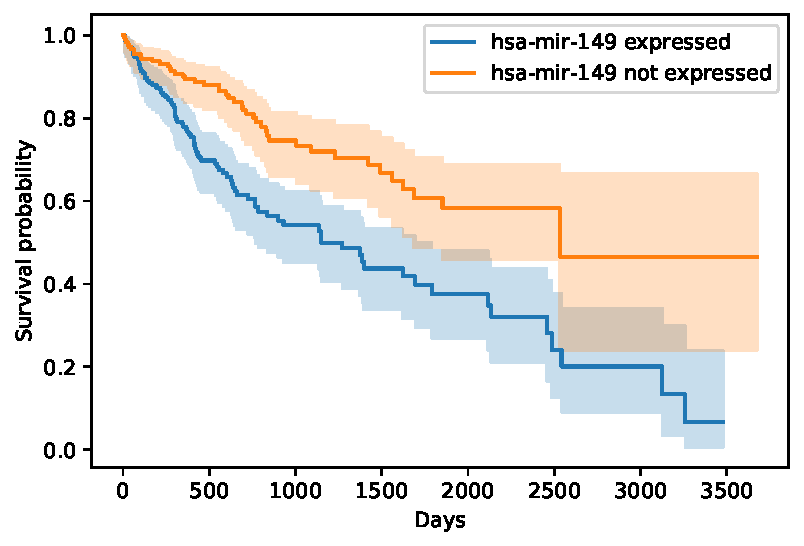
\includegraphics[width=0.48\textwidth]{hsa-mir-149}\hfill
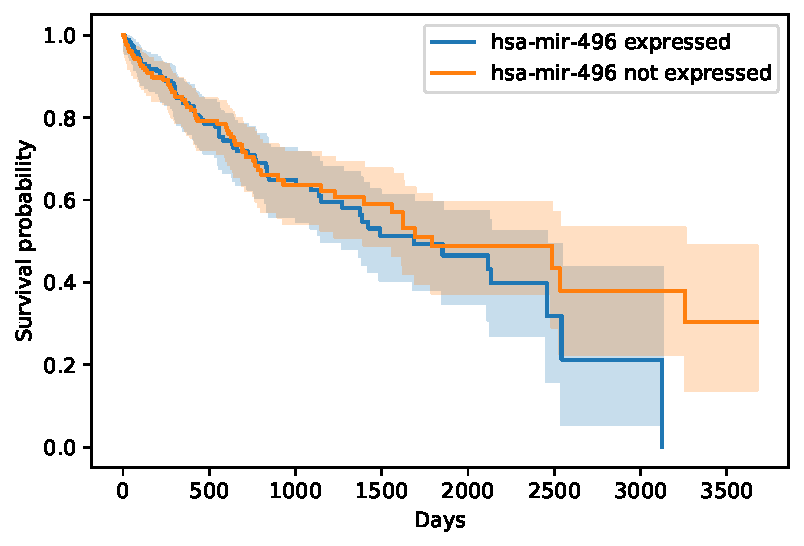
\includegraphics[width=0.48\textwidth]{hsa-mir-496}
\caption{An example of a Kaplan-Meier plot for two gene expression-dependent conditions associated with patient survival. In panel a), the survival function is substantially higher for a group of patients with highly expressed microRNA hsa-mir-149. The difference is not so evident in the panel b) and microRNA hsa-mir-496. We could say that hsa-mir-149 is hence a better biomarker for survival. In biomarker discovery, one of the tasks is to rank genes and RNA molecules according to the degree of separation between corresponding survival signatures when a gene is expressed and not expressed.}
\label{fig:km-marker}
\end{figure}

\bold{Ideally, therefore, data-driven discovery of new biomarkers would only require survival data with gene expression profiles of target tissues for patients or cell cultures with variety of outcomes and treatments.} The discovery algorithms would then sip through all the genes and find those that best define groups with different survival function. But there are many difficulties and obstacles in this procedure, related to noisy data, small datasets in terms of the number of investigated samples, higher-order gene interactions, and inclusion of available additional knowledge. We examine these more closely next.

\subsubsection*{Problem Description}

\bold{There are three category of problems and challenges we would like to address in the proposed project, affecting the computation methods to infer potential biomarkers, approaches to data fusion, and implementation aspects:}
\begin{description}
	\item[Computational challenges, noise and overfitting.] The experimental data that addresses a specific survival problem, related to, say, impact of a new treatment or drug, is often expensive and hence small in sample size due. Experimental noise related to sample collection and treatment, and to measurement of gene expression can be high. This setting can lead to false discoveries and overfitting. The problem is especially exposed when finding sets, or networks of genes that could serve as biomarkers, as the number of candidates (different sets of genes) grows exponentially with the desired size of the gene set. For instance, with $20.000$ genes, there are over $1,3$ trillion possible gene triples; even if we would computationally manage to examine them all, checking so many combinations will necessary lead to overfitting, where our results would apply well to the training data, but not generalize well to new cases. Besides noise and overfitting, computational challenges include those in finding gene expression thresholds (when is a gene expressed?) and aggregation functions (when is a set of genes collectively active?).
	\item[Inclusion ob background knowledge.] Genes participate in molecular pathways, perform functions, and are associated to diseases and responses to chemicals and drugs. Knowledge about these and other gene annotations is stored in data bases such as GeneOntology~\cite{}, KEGG~\cite{}, PathwayCommons~\cite{}, CellMarker~\cite{}, and other. Examining gene sets as candidates for biomarkers could and should use these valuable sources of information, both for restricting the biomarker search space and interpreting the sets of best candidate genes. Such fusion of data and knowledge bases has been at culprit of bioinformatics research~\cite{} but has been insufficiently explored in our target domain of survival biomarker discovery.
	\item[Data exploration interface.] The past two decades have seen an emergence of a wide array of methods and statistical and machine learning tools to analyze high-throughput data from molecular biology. For survival analysis, however, there is no elegant toolbox with an intuitive user interface that would assist in biomarker discovery, support on-the-fly interactive exploratory data analysis, and offer easy construction of analytical pipelines. Available are excellent code libraries for survival analysis in R and Python, yet, for a systematic use, these are just building blocks whose joint utility and integration requires advanced knowledge of programming. What we need instead are intuitive tools with flexible and exciting interactive interfaces to engage the end-users and data scientists in productive communication, data exploration and modeling.
\end{description}

\bold{In the project, we will address these three challenges through development of techniques and tools that will support interactive search for and exploration of potential biomarkers.} We aim to democratize the field of data-driven biomarker discovery by creating a versatile tool with interactive interface for intelligent analysis of survival data.

\subsubsection*{Project Aims}

{\ bf The project will develop and apply a set of computational tools for inference of biomarkers from survival data.} We will integrate existing approaches to survival data-based biomarker scoring, survival modeling, and gene set enrichment analysis, and propose new techniques for survival-specific gene interactions, construction of biomarker candidate maps, and interpretation of constructed visualizations. We will devise means for heuristic search that will use published data bases on gene function and pathway annotation.

{\em The project will address the means by which domain experts and data miners use these tools in real-life applications.} The project will embed computation methods in components with graphical user interfaces. We will enhance our own, open-source data mining platform Orange~\footnote{\url{http://orangedatamining.com}} with survival analysis capabilities. We will show that the resulting visual programming platform not only substantially reduces the complexity and user time spent on data analysis, but also enhances the collaboration and motivation of domain experts through informative visualizations and ability to steer the discovery process using domain knowledge. 

{\em Finally, we would like to showcase the utility of the constructed toolbox.} In the application of project's approaches we will use a set of published and privately-owned (from participating SME) datasets on drug response and cancer. The success of the project will be judged on use cases carried out by participating SME, and our ability to train them to independently use the results of the project.

\subsubsection*{Anticipated Results}
The expected principal results of this project are:
\begin{enumerate}
	\item bioinformatics library to support biomarker discovery from survival data. The library will be developed in Python and will be published in open-source on GitHub, together with documentation, unit-tests, and working examples;
	\item a biomarker discovery toolbox featuring visual programming interface, interactive visualizations, and means of interpretation and explanation of results. The toolbox will support integration of external knowledge-bases, on-the-fly construction of analytical pipelines, and domain knowledge-based guided data exploration;
	\item a set of use-cases developed in close collaboration with Genialis, an participating SME. The use-cases will demonstrate the applicability of our software, showcase the power of toolbox's intuitive interface, and provide for instruction and educational material in dissemination of project's results.
\end{enumerate}

\subsubsection*{Preliminary Results and Studies}

gene network discovery, gene interactions, intelligent data visualization, embedding, Orange.

\subsection{State-of-the-art in the proposed field of research and survey of the relevant literature}

Intro paragraph.

\subsubsection*{Computation Methods for Gene Markers Identification in Survival Analysis}
\subsubsection*{Visual Data Analysis}
\subsubsection*{Toolboxes}

\subsection{Detailed Description of the Work Programme}

\subsubsection{Project Tasks}

The project will be organized around a following set of tasks:
\begin{description}
	\item[T0] \bold{Setting-up of the collaborative environment.} We will deposit all the code and documentation on GitHub~\footnote{\url{https://github.com/biolab}}. The repository will store project documentation and meeting minutes, tasks management through creation and tracking of issues, Python library code, unit-test, and examples. Data files will be stored on a separate web server. Extensions of Orange~\footnote{\url{https://orangedatamining.com}} will be developed as an add-on and will be stored in a separate repository on the GitHub.
	\item[T1] \bold{Data acquisition and organization.} The project will use a number of different data sets coming from published studies and databases such as NCBI's Gene Expression Omnibus~\footnote{\url{https://www.ncbi.nlm.nih.gov/geo/}} and TCGA, The Cancer Genome Atlas database~\footnote{\url{https://portal.gdc.cancer.gov}}. In addition we will also create a set of synthetic data sets of varying size and complexity. The compiled data sets will be stored in our own dataset repository created in task T1.
	\item[T2] \bold{Development of data mining and bioinformatics for survival biomarker discovery.} In particular, we will develop and implement techniques for:
	\begin{description}
		\item[T2.1] \bold{Survival function-based gene ranking and selection}, where we will implement standard techniques from the field, including the log rank test~\cite{} and the ranking based on the inference of Cox proportional hazards model. We will also include more recent and advanced modeling approaches based on bootstrap~\cite{} and deep learning~\cite{}, and infer gene ranking through studying the sensitivity of the models~\cite{}.
		\item[T2.2] \bold{Feature construction}, where we will use predictive models on a smaller subset of genes to aggregate gene expression and with this aim to increase the robustness of so-inferred biomarker. We will employ $\ell^0$ regularization in combination with Cox and derived models, and network-based approaches where biomarker is composed of a small number of genes from the same network community~\cite{}.
		\item[T2.3] \bold{Gene interaction analysis}, where we expect that a group of genes can interact in a non-linear way to form a more robust and informative biomarker. We will adapt the approaches for finding feature interactions~\cite{} to address survival data, and the approaches to visualize the results of interaction analysis~\cite{}.
		\item[T2.4] \bold{Knowledge-infused biomarker discovery}, where we will restrict the search space of survival-effecting gene interactions to groups of genes with shared functional annotations from knowledge libraries on gene annotations, pathways, and known markers.
		\item[T2.5] \bold{Deep and transfer learning}, where our aim is to find gene embeddings for their profiling in low-dimensional space. We will use auxiliary dataset to train variational autoencoders~\cite{} for embedding, and then adapt the embedding to specific survival problem using transfer learning~\cite{}, that is, modifying only a small part of the deep model. We will use the embedded, latent profiles of genes for visualizations of gene maps and in heuristics to restrict the search space.
		\item[T2.6] \bold{Gene interaction maps}, where we would like to represent genes -- potential biomarkers -- in a gene map where vicinity of genes on the map suggest increased joint effect on the survival function. The constructed interaction plots will serve for mapping of interaction space and presentation of the space of solutions to biomarker discovery problem.
		\item[T2.7] \bold{Automatic annotation of point-based visualizations}, where points are genes and a primary example of such visualizations are gene interaction maps. We will devise algorithms that search for visualization neighborhoods with enriched gene function or pathways, and annotate visualizations accordingly. This research will follow our prior work on annotation of gene maps for single-cell analysis~\cite{}.
	\end{description}
	\item[T3] \bold{Design of visual interfaces for exploratory analysis of survival data and biomarker discovery.} We will design components and pipelines for interactive, domain-knowledge driven mining of biomarkers from survival-related gene expression data. The design will include the planning of a set of computational components to address all aspects of survival analysis and biomarker discovery. We will design the graphical interface of the components, their visual presentation, interactive visualizations, and possible data analysis pipelines to combine the design components. The deliverable will include sketches of graphical user interface (in Balsamiq Mockups) and wire-frames. The design will emphasize the quality of user experience, access to advanced computational techniques, and ability to combine components in a Lego-brick way to devise possibly complex and powerful analysis pipelines.
	\item[T4] \bold{Implementation and Integration.} Computational techniques we will develop in the project will be implemented within an open-source data mining environment Orange\footnote{\url{http://orangedatamining.com})}. The implementation will use the library of methods from task T2 and graphical user designs from T3. Implementations will be released as an separate add-on to Orange, and will follow implementation guidelines, which refer to documentation, and unit testing with near 100\% code coverage.
	\item[T5] \bold{Experimental validation}, where we will closely collaborate with Genialis, our project partner, to thoroughly test the functionality of implemented toolbox on synthetic and real data sets. The results will be compared to those from the literature. Experimental validation will use the data sets prepared in task T1. The validation will confirm the validity and corectness of developed procedures and will serve to collect case studies to be published in material we will post on GitHub, Orange's web site, and in planned publications.
	\item[T6] \bold{Dissemination of results,} which includes publishing of the implementation of the developed methods under General Public License (GPL), writing and web-publishing of relevant documentation with working examples, publishing video tutorials with use cases on Orange's YouTube channel\footnote{\url{http://youtube.com/orangedatamining}}, and dissemination in terms of presentation at relevant conferences and journal publications. We will target bioinformatics journals, such as {\em Bioinformatics}, {\em Nature Methods}, and {\em Artificial Intelligence in Medicine}, and related conferences including top-rated AIM and ISMB.
\end{description}

\subsubsection{Research Design and Methods}
\begin{description}
	\item[Overview.] 
The overview of the research in the proposed project is presented in Figure~\ref{fig:approach}. The figure shows how we will integrate existing and new experimental data on genetic interactions, whole genome gene expression data sets, and data on cytotoxicity to find:
1. which genes are functionally related to a particular drug, or to a class of drugs with common characterization,
2. what is the mechanism through which a set of drugs causes cytotoxic effects,
3. which other experiments could further improve the reliability of the inferred hypothesis on drug action.
While all of the above are clearly the issues to be addressed by a biomedical engineer, due to sheer volume of data and additional information in available data and knowledge they can only be addressed through means of computational analysis and discovery approaches. The principal challenge of the project is how to combine these different sources, and use modern data mining approaches to support knowledge discovery to provide interpretable and operational hypotheses to biomedical researchers and drug developers. In the description below, we first describe the data on which our drug characterization and discovery process will be based, then enlist a set of computational approaches which we will develop and use, comment on their implementation within an existing visual programming-based data mining framework, and integration in robotic experimental chemical genomics platform.

\begin{figure}
\floatbox[{\capbeside\thisfloatsetup{capbesideposition={right,top},
capbesidewidth=0.4\textwidth}}]{figure}[\FBwidth]
{\caption{An example of a Kaplan-Meier plot for two gene expression-dependent conditions associated with patient survival. In panel a), the survival function is substantially higher for a group of patients with highly expressed microRNA hsa-mir-149. The difference is not so evident in the panel b) and microRNA hsa-mir-496. We could say that hsa-mir-149 is hence a better biomarker for survival. In biomarker discovery, one of the tasks is to rank genes and RNA molecules according to the degree of separation between corresponding survival signatures when a gene is expressed and not expressed.}\label{fig:test}}
{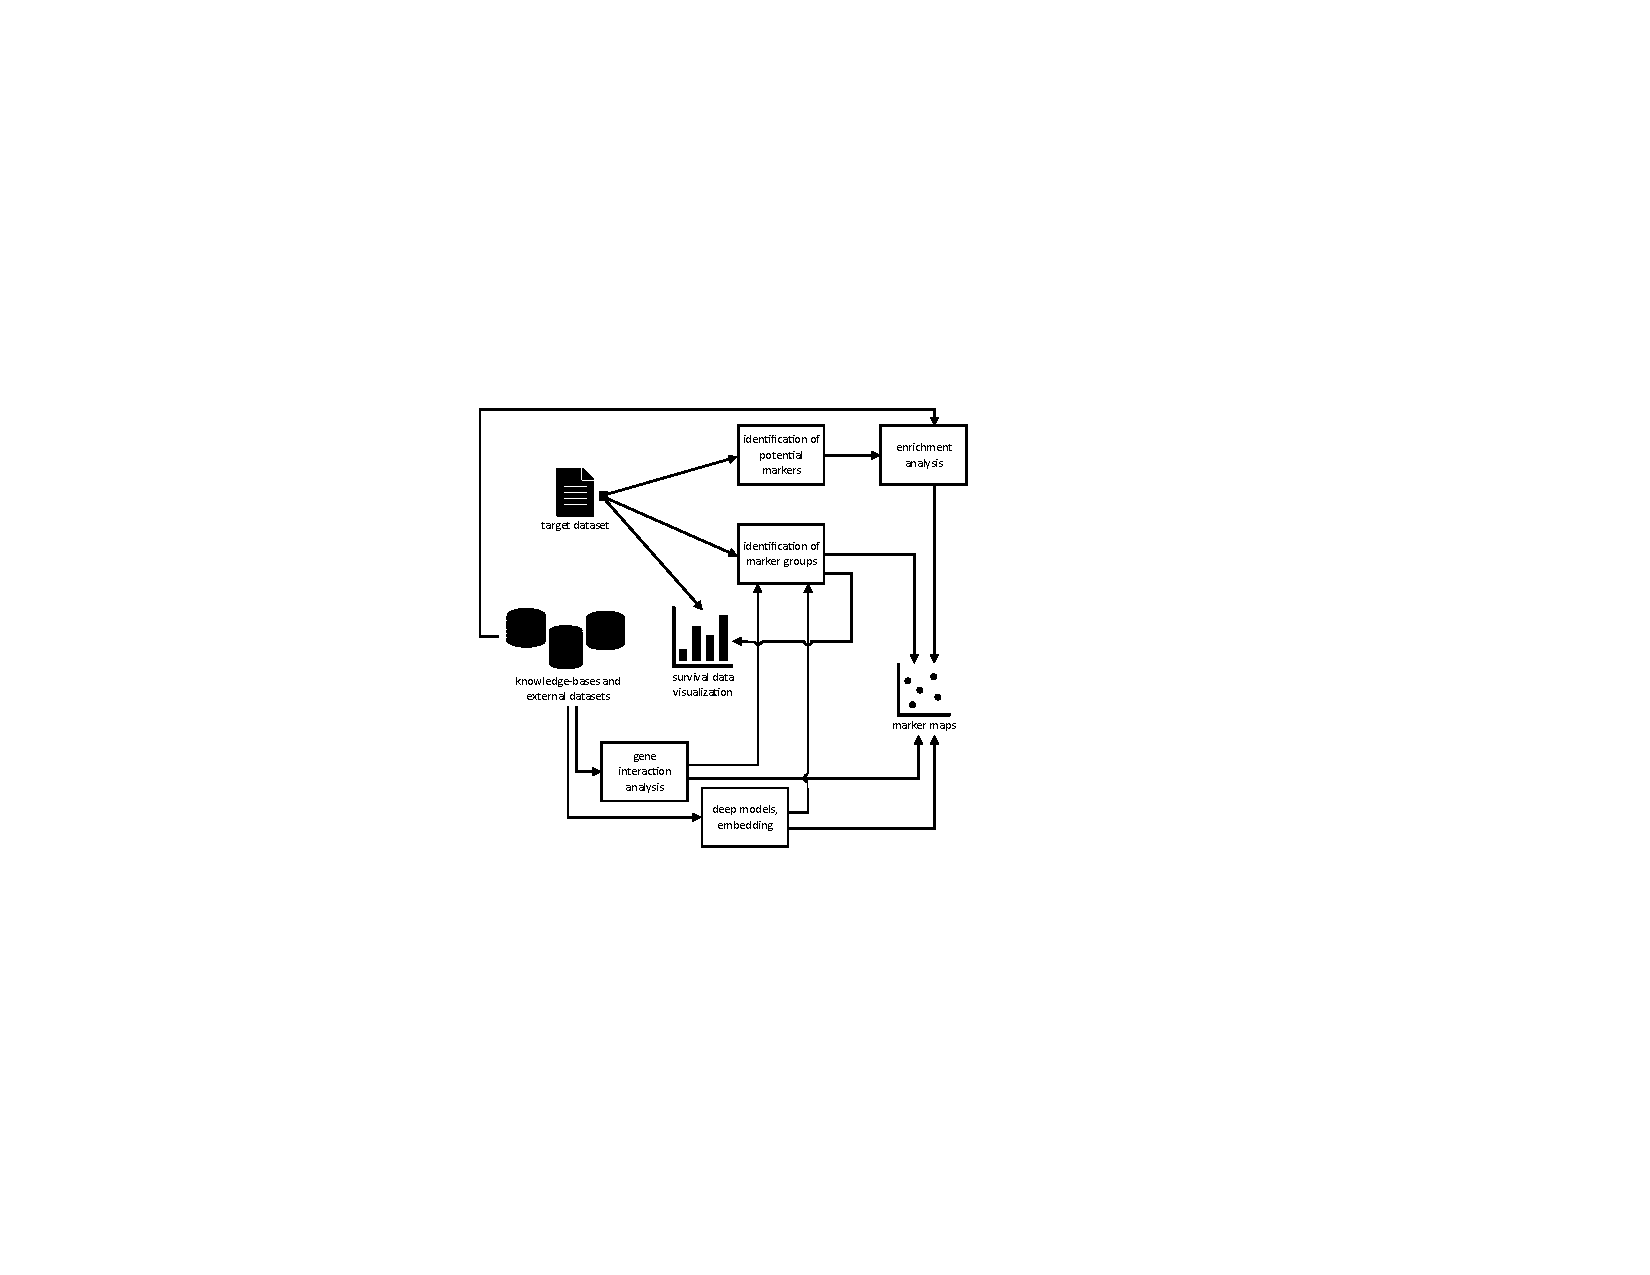
\includegraphics[width=0.6\textwidth]{approach}}
\end{figure}


% \begin{figure}
% 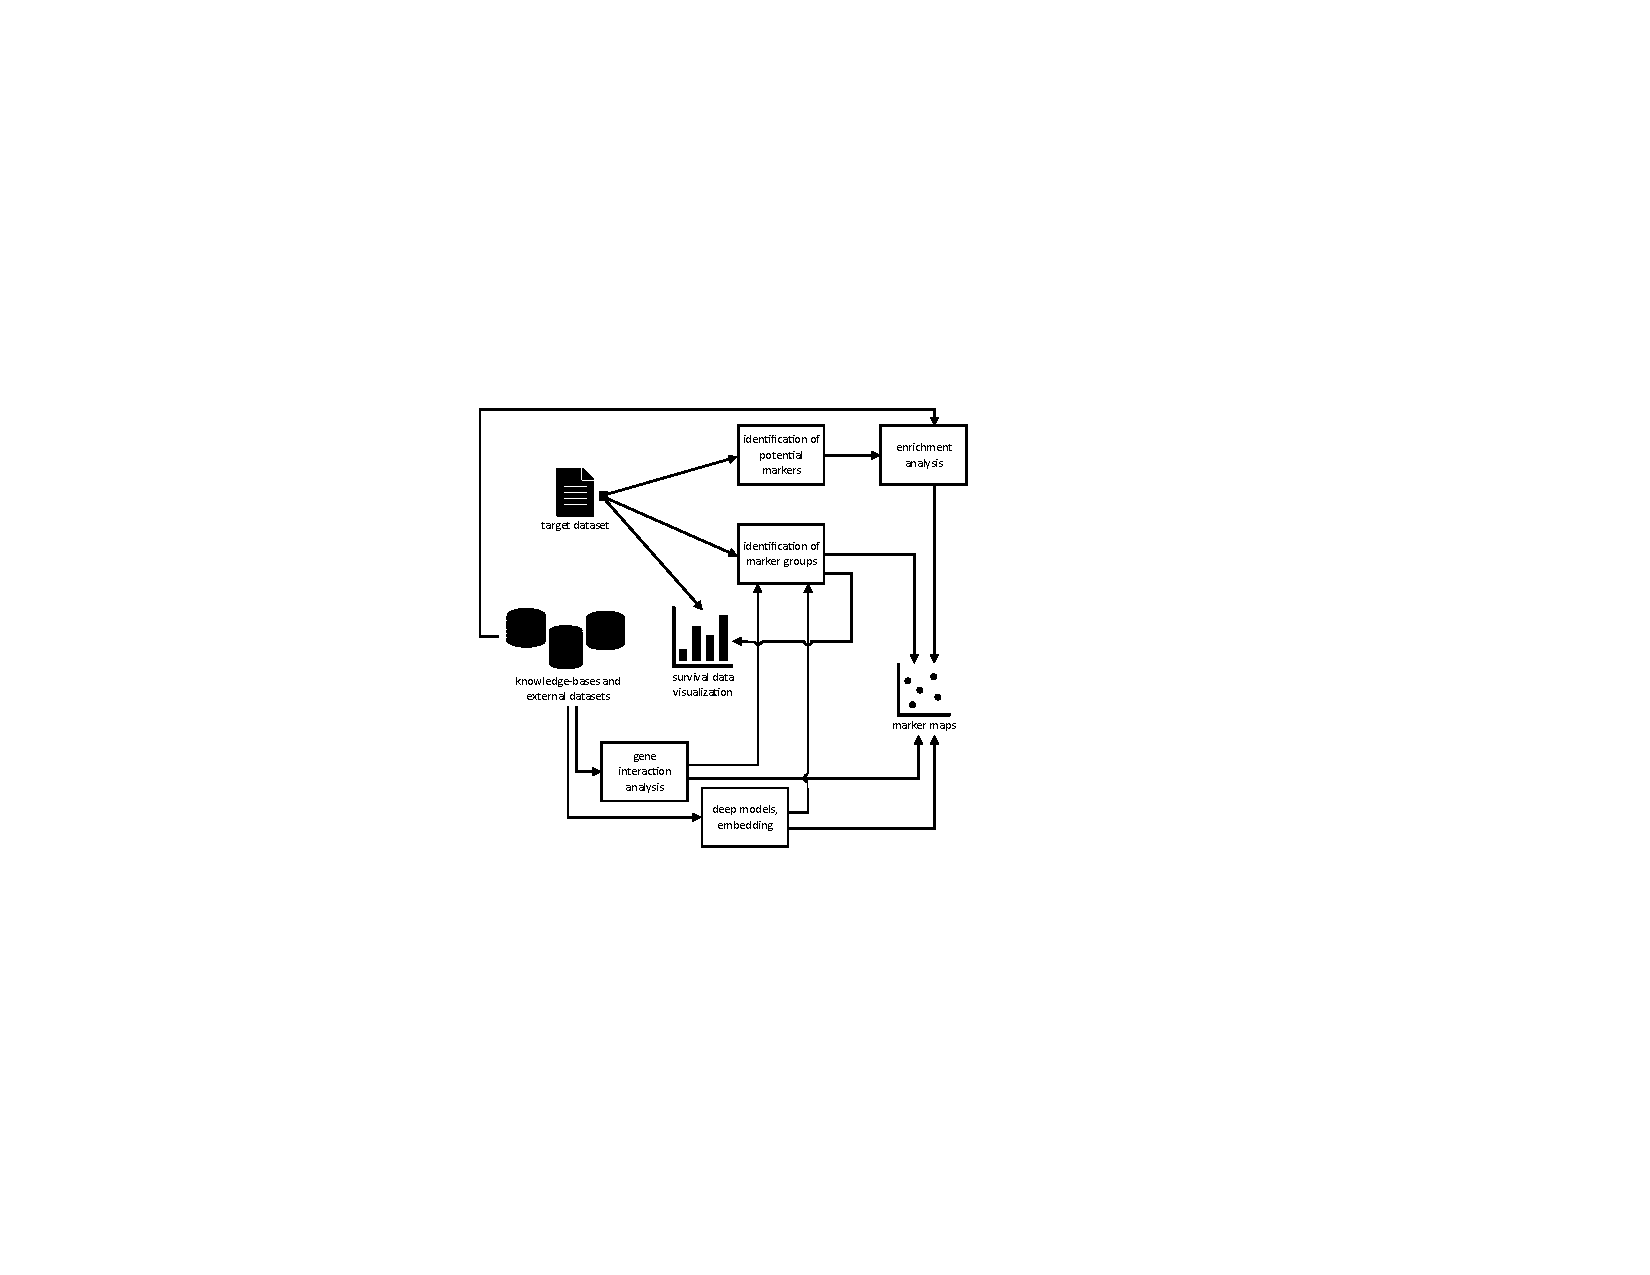
\includegraphics[width=0.48\textwidth]{approach}
% \caption{An example of a Kaplan-Meier plot for two gene expression-dependent conditions associated with patient survival. In panel a), the survival function is substantially higher for a group of patients with highly expressed microRNA hsa-mir-149. The difference is not so evident in the panel b) and microRNA hsa-mir-496. We could say that hsa-mir-149 is hence a better biomarker for survival. In biomarker discovery, one of the tasks is to rank genes and RNA molecules according to the degree of separation between corresponding survival signatures when a gene is expressed and not expressed.}
% \label{fig:approach}
% \end{figure}


	\item[Material and Data Sets.] Text here.
	\item[Computational Approaches, Data Mining and Bioinformatics.] Text here.
	\item[Software Implementation.] Text here.
	\item[Experimental Validation.] Text here.
\end{description}

\subsection{Available research equipment over 5.000 €}

\subsection{Project management}
% Detailed implementation plan and timetable
% gantt
% risks and remedies

\end{document}